\chapter{Phép quay, spinor và đối xứng màu}

\section{Các phép quay như một nhóm}

Các phép quay trong không gian là những đối xứng, và chúng tác dụng lên nhiều loại đối tượng. Chúng tác dụng lên vật rắn, lên các vectơ vận tốc, lên các trường vectơ và lên các trạng thái lượng tử. Một vectơ thông thường là điểm khởi đầu đơn giản nhất vì phép biến đổi của nó có thể được hình dung trực tiếp.

Các phép quay cũng có thể được tổ hợp. Hãy quay một vật quanh một trục qua một góc, rồi sau đó quay nó quanh trục thứ hai qua góc thứ hai. Định hướng cuối cùng tương đương với một phép quay duy nhất quanh một trục thứ ba nào đó qua một góc thứ ba nào đó. Vì vậy tích của hai phép quay lại là một phép quay khác.

Tích này là một phép toán trên các phép biến đổi, không phải là phép cộng của hai vectơ trục. Phép quay thứ nhất làm thay đổi đối tượng mà phép quay thứ hai tác dụng lên. Nếu \(R_1\) được thực hiện trước và \(R_2\) sau đó, thì phép toán kết hợp được viết là \(R_2R_1\). Bản thân nó là một \(R_3\) nào đó, mặc dù việc tìm trục và góc của \(R_3\) có thể bất tiện. Tính đóng dưới phép hợp thành này là lý do đầu tiên để xem các phép quay như một nhóm chứ không chỉ đơn thuần là một danh sách các chuyển động hình học.

Trước hết, sẽ hữu ích nếu mô tả một phép quay theo hình học. Chọn một vectơ đơn vị \(\hat{\boldsymbol n}\) dọc theo trục quay và một góc \(\theta\). Ta dùng quy ước bàn tay phải. Một phép quay theo quy tắc tay trái qua \(\theta\) cũng có thể được viết như một phép quay theo quy tắc tay phải qua \(-\theta\), hoặc như một phép quay theo quy tắc tay phải quanh \(-\hat{\boldsymbol n}\).

\begin{figure}[htbp]
\centering
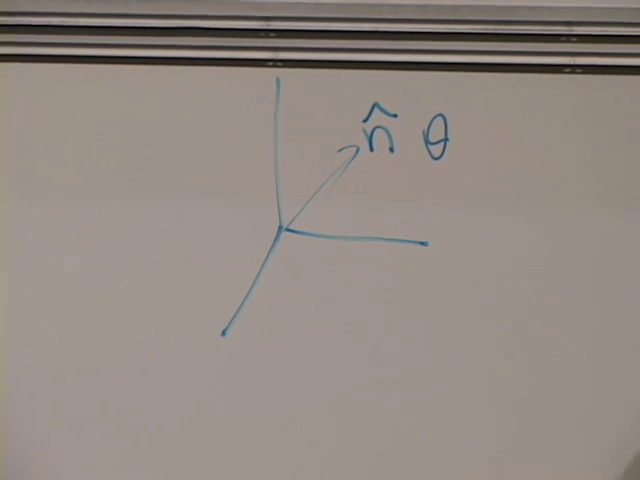
\includegraphics[width=0.58\textwidth]{lecture_03_figure_02.png}
\caption{Một trục \(\hat{\boldsymbol n}\) và một góc \(\theta\) xác định một phép quay trong không gian.}
\lectureframe{00:02:34}
\end{figure}

Một hướng trên mặt cầu đơn vị cần hai tham số, chẳng hạn như kinh độ và vĩ độ. Góc quay quanh hướng đó cung cấp tham số thứ ba. Do đó, các phép quay tạo thành một họ ba tham số. Tạm thời ta chưa cần bận tâm đến các đồng nhất hóa toàn cục do những góc sai khác nhau một \(2\pi\) gây ra; điều quan trọng ở đây là số lượng tham số cục bộ.

Mô tả bằng trục và góc có một chút dư thừa. Đảo ngược trục đồng thời đảo dấu góc cho cùng một phép toán, và những góc đủ lớn có thể được rút gọn theo modulo một vòng tròn đầy đủ. Không điều nào trong số đó làm thay đổi sự thật rằng gần phép đồng nhất, một phép quay có ba tham số biến thiên liên tục. Về sau, số đếm cục bộ ấy sẽ được đối chiếu với số tham số độc lập trong một biểu diễn ma trận.

Các tính chất của nhóm giờ đây có thể được kiểm tra lần lượt:
\begin{enumerate}
\item \emph{Tính đóng.} Thực hiện liên tiếp hai phép quay tạo ra một phép quay khác.
\item \emph{Phần tử đơn vị.} Không làm gì cả là phép quay đồng nhất.
\item \emph{Nghịch đảo.} Một phép quay qua \(\theta\) quanh \(\hat{\boldsymbol n}\) được hoàn tác bởi một phép quay qua \(-\theta\) quanh cùng trục đó.
\item \emph{Tính kết hợp.} Ba phép quay liên tiếp thỏa mãn
\[
(R_1R_2)R_3=R_1(R_2R_3).
\]
\end{enumerate}

Các phép quay không giao hoán. Một phép quay quanh trục \(x\) rồi tiếp theo là một phép quay quanh trục \(y\) nói chung cho một định hướng khác với khi thực hiện cùng hai phép toán ấy theo thứ tự ngược lại:
\begin{equation}
R_x(\alpha)R_y(\beta)\ne R_y(\beta)R_x(\alpha).
\end{equation}
Sự khác biệt trở thành bậc hai khi cả hai góc đều rất nhỏ, đó là lý do vì sao các phép quay vi phân có thể trông gần như giao hoán. Tuy vậy, toàn bộ nhóm vẫn là không abel.

Tính không giao hoán có thể được kiểm tra mà không cần bất kỳ phương trình nào. Hãy lấy một quyển sách hoặc một cái hộp, đánh dấu một mặt là mặt trước, rồi xoay nó chín mươi độ quanh trục \(x\) và sau đó chín mươi độ quanh trục \(y\). Trở về định hướng ban đầu và đảo ngược thứ tự. Mặt đã đánh dấu sẽ kết thúc theo một hướng khác. Với các góc nhỏ, độ sai khác khó thấy hơn, nhưng nó không biến mất; nó bắt đầu ở tích của hai góc nhỏ ấy.

\begin{classroomqa}
\audiencequestion{Các phép quay này là tuần tự chứ không phải đồng thời, đúng không?\lecturetimestamp{00:04:45}}
\lecturerresponse{Đúng. Phép nhân nhóm có nghĩa là một phép toán theo sau bởi một phép toán khác. Chính thứ tự của những phép quay liên tiếp ấy là điều có thể không giao hoán.}
\end{classroomqa}

Đây là nhóm không abel đầu tiên của chúng ta. Ứng dụng sau cùng không phải là màu của một vật thông thường mà là các trạng thái màu đỏ, lục và lam của một quark. Đó là một hệ nội tại ba trạng thái, và những phép biến đổi đáng quan tâm của nó trộn lẫn ba màu ấy. Các phép quay thông thường cung cấp một mô hình quen thuộc về cách một nhóm liên tục tác dụng thông qua các ma trận.

Bản thân một nhóm là trừu tượng. Để sử dụng nó trong vật lý, ta phải nói nó tác dụng lên những đối tượng nào. Một {biểu diễn} gán cho mỗi phần tử của nhóm một toán tử hoặc ma trận sao cho phép nhân các phần tử nhóm được tái hiện bởi phép nhân của các ma trận được gán. Những đối tượng vật lý khác nhau có thể mang những biểu diễn khác nhau của cùng một nhóm. Vectơ, các trạng thái spin một và các trạng thái spin một nửa sẽ cung cấp ba ví dụ.

\section{Biểu diễn vectơ ba chiều}

Cho một vectơ thông thường có các thành phần
\begin{equation}
\boldsymbol V=(V_x,V_y,V_z),\qquad V_i,\quad i=1,2,3.
\end{equation}
Ta có thể quay vectơ vật lý trong khi giữ cố định các trục, hoặc quay các trục tọa độ trong khi giữ cố định vectơ. Các quy ước là khác nhau, nhưng trong cả hai cách mô tả, các thành phần đều bị trộn bởi một ma trận \(3\times3\). Với mọi cặp trục-góc \((\hat{\boldsymbol n},\theta)\), viết
\begin{equation}
V_i'=R_{ij}(\hat{\boldsymbol n},\theta)V_j,
\label{eq:l3-vector-rotation}
\end{equation}
trong đó chỉ số lặp được lấy tổng.

Chỉ số lặp \(j\) là một nhãn giả. Phương trình ~\eqref{eq:l3-vector-rotation} có nghĩa tường minh là
\begin{equation}
V_i'=R_{i1}V_1+R_{i2}V_2+R_{i3}V_3
\end{equation}
cho mỗi thành phần đầu ra \(i\). Chỉ số tự do \(i\) cho biết thành phần nào đang được tính; \(j\) lặp được lấy tổng và có thể đổi tên mà không làm thay đổi phương trình. Giữ tách biệt hai vai trò đó sẽ ngăn được phần lớn các sai sót về chỉ số trong lập luận bảo toàn độ dài.

\begin{figure}[htbp]
\centering
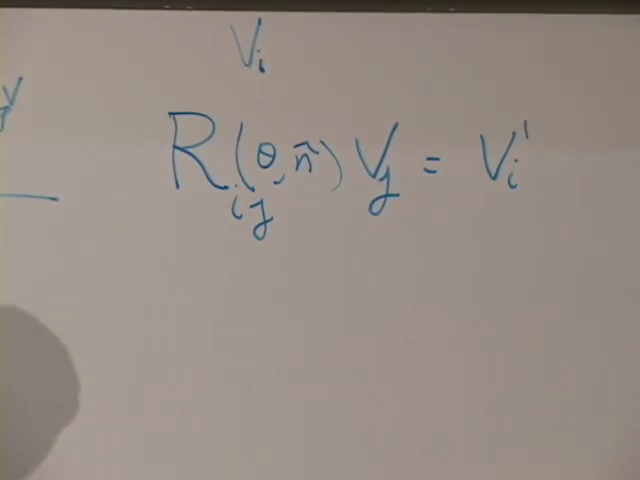
\includegraphics[width=0.68\textwidth]{lecture_03_figure_03.png}
\caption{Ma trận quay ánh xạ các thành phần vectơ ban đầu thành các thành phần sau khi quay.}
\lectureframe{00:07:41}
\end{figure}

Một phép quay đúng nghĩa bảo toàn độ dài. Tạm thời cả \(V_i\) lẫn \(R_{ij}\) đều là số thực, nên
\begin{equation}
V_i'V_i'=V_iV_i
\end{equation}
đúng với mọi vectơ. Để làm rõ điều kiện đối với ma trận, hãy viết cùng phép biến đổi đó với các chỉ số giả khác nhau:
\begin{equation}
V_i'=R_{ij}V_j,\qquad V_i'=R_{ik}V_k.
\end{equation}
Nhân rồi lấy tổng theo \(i\) cho ta
\begin{align}
V_i'V_i'
 &=R_{ij}V_jR_{ik}V_k\\
 &=R_{ij}R_{ik}V_jV_k.
\end{align}
Biểu thức này bằng \(V_jV_j\) với mọi lựa chọn của \(V\) chỉ khi
\begin{equation}
R_{ij}R_{ik}=\delta_{jk}.
\label{eq:l3-orthogonality-index}
\end{equation}
Trong ký hiệu ma trận,
\begin{equation}
R^TR=\boldsymbol 1,
\label{eq:l3-orthogonal}
\end{equation}
và do đó
\begin{equation}
R^{-1}=R^T.
\end{equation}
Phép chuyển vị chỉ đơn giản là hoán đổi hàng và cột.

Vì sao hệ số phải là \(\delta_{jk}\)? Delta Kronecker buộc \(j=k\) trong phép lấy tổng:
\begin{equation}
\delta_{jk}V_jV_k=V_1^2+V_2^2+V_3^2.
\end{equation}
Nếu \(R_{ij}R_{ik}\) khác \(\delta_{jk}\), thì một hướng nào đó hoặc một hạng chéo nào đó \(V_jV_k\) sẽ làm thay đổi độ dài. Vì đẳng thức này được yêu cầu đúng với mọi vectơ có thể có, chứ không chỉ với một vectơ được chọn, nên bản thân hệ số ma trận phải bằng ma trận đơn vị.

Phương trình ~\eqref{eq:l3-orthogonal} là điều kiện trực giao định nghĩa cho biểu diễn ma trận thực này. Phép nhân các ma trận tái hiện bảng nhân của các phép quay trong không gian. Đây không phải là biểu diễn duy nhất của nhóm quay; nó chỉ đơn thuần là biểu diễn dễ hình dung nhất.

Quan hệ nghịch đảo có một ý nghĩa hình học trực tiếp. Một phép quay có thể được hoàn tác mà không cần giải một phương trình ma trận mới: chỉ việc đổi hàng với cột. Nếu \(R_1\) và \(R_2\) biểu diễn hai phép quay, thì \(R_2R_1\) biểu diễn tác dụng liên tiếp của chúng và lại là trực giao. Vì vậy, các phép toán ma trận bảo toàn đúng cùng cấu trúc đóng, đơn vị, nghịch đảo và kết hợp đã được xác lập về mặt hình học.

\section{Spin một và biểu diễn vectơ}

Biểu diễn ba chiều cũng tác dụng lên các trạng thái lượng tử. Một hạt spin một có ba hình chiếu spin khả dĩ,
\begin{equation}
m=+1,\quad 0,\quad -1.
\end{equation}
Do đó, trạng thái spin của nó là một cột ba thành phần của các biên độ xác suất. Quay hạt, hoặc thay đổi định hướng của từ trường dùng để xác định trục spin, sẽ trộn ba biên độ ấy bởi một biểu diễn ba chiều của nhóm quay.

Số trạng thái spin tuân theo quy tắc quen thuộc \(2s+1\). Spin không có một trạng thái, spin một nửa có hai, spin một có ba, và spin ba phần hai có bốn. Vì vậy, số chiều của vectơ trạng thái thay đổi theo spin. Cùng một phép quay vật lý phải được biểu diễn bằng các ma trận có kích thước khác nhau khi nó tác dụng lên các không gian trạng thái khác nhau này.

Đối với một hạt spin một, hãy chọn cơ sở
\begin{equation}
\lvert 1,+1\rangle,qquad
\lvert 1,0\rangle,qquad
\lvert 1,-1\rangle.
\end{equation}
Một trạng thái là
\begin{equation}
\lvert\psi\rangle
=c_{+}\lvert1,+1\rangle+c_0\lvert1,0\rangle+c_{-}\lvert1,-1\rangle.
\end{equation}
Việc quay thiết bị không tạo ra trạng thái spin thứ tư; nó trộn ba hệ số \(c_+,c_0,c_-\) với nhau. Vì thế, toán tử quay tương ứng phải là một ma trận \(3\times3\).

Đối với spin một, biểu diễn này biến đổi theo cùng cách như một vectơ không gian thông thường. Đó là ý nghĩa chính xác của việc gọi một hạt spin một là hạt \emph{vectơ}: ba biên độ spin của nó và ba thành phần của một vectơ tuân theo cùng một quy luật quay. Không cần hình dung trạng thái lượng tử như một mũi tên theo nghĩa đen; phát biểu này nói về cách các thành phần của nó bị trộn lẫn.

Sự tương ứng này không phải là ngẫu nhiên. Một vectơ ba chiều và một trạng thái spin một mang các biểu diễn ba chiều tương đương của nhóm quay. Cụm từ {hạt vectơ} tóm tắt tính chất biến đổi đó. Nó không hề khẳng định rằng một trạng thái phân cực lượng tử là một mũi tên cứng tí hon ẩn bên trong hạt.

\section{Đối xứng rời rạc và liên tục}

Trước khi chuyển sang spin một nửa, sẽ hữu ích nếu phân biệt hai loại nhóm rộng. Một phép phản xạ cho một ví dụ rời rạc đơn giản. Có phép đồng nhất và có phép phản xạ \(P\); hoặc ta lật, hoặc không lật. Trái lại, một pha
\begin{equation}
e^{i\phi}
\end{equation}
phụ thuộc liên tục vào \(\phi\), và một phép quay trong không gian phụ thuộc liên tục vào trục và góc của nó. Những nhóm liên tục như vậy được gọi là \emph{nhóm Lie}, theo tên Sophus Lie; tên ấy được phát âm là \emph{Lee}. Các đối xứng liên tục sẽ là mối quan tâm chính, mặc dù các đối xứng rời rạc vẫn quan trọng.

Đối với nhóm phản xạ hai phần tử,
\begin{equation}
P^2=1.
\end{equation}
Không có một mức độ phản xạ nào điều chỉnh liên tục được giữa \(1\) và \(P\). Nhóm pha thì khác: giữa \(e^{i\phi_1}\) và \(e^{i\phi_2}\) có liên tục vô số pha khác. Các phép quay trong không gian có cùng tính liên tục đó, nhưng khác với \(U(1)\), chúng là không abel.

Spin không cho biểu diễn đơn giản nhất của nhóm quay. Một trạng thái spin-không không đổi dưới mọi phép quay, nên mỗi phần tử nhóm đều được biểu diễn bởi đồng nhất một chiều:
\begin{equation}
D^{(0)}(R)=1.
\end{equation}
Bản thân nhóm vẫn có vô số phép quay; chính biểu diễn trên trạng thái spin-không mới là tầm thường.

Sự phân biệt này giữa một nhóm và một trong các biểu diễn của nó là cốt yếu. Nhóm quay không suy sụp thành một nhóm một phần tử mỗi khi nó tác dụng lên một vô hướng. Đúng hơn, mọi phần tử của nó đều được biểu diễn bởi cùng một số \(1\) trên trạng thái vô hướng cụ thể đó.

\section{Một trạng thái spin một nửa tổng quát}

Một hệ spin một nửa có hai trạng thái cơ sở. Đối với một trục \(z\) đã chọn,
\begin{equation}
\lvert\uparrow\rangle=
\begin{pmatrix}1\\0\end{pmatrix},
\qquad
\lvert\downarrow\rangle=
\begin{pmatrix}0\\1\end{pmatrix}.
\end{equation}
Một trạng thái tổng quát là một spinor hai thành phần,
\begin{equation}
\lvert\psi\rangle=
\begin{pmatrix}\alpha_1\\\alpha_2\end{pmatrix},
\qquad
|\alpha_1|^2+|\alpha_2|^2=1.
\label{eq:l3-spinor}
\end{equation}
Các thành phần là số phức. Lựa chọn \((\alpha_1,\alpha_2)=(1,0)\) là spin lên, và \((0,1)\) là spin xuống. Một tổ hợp chuẩn hóa tổng quát mô tả một spin được phân cực dọc theo một hướng nào đó khác.

Các từ {lên} và {xuống} chỉ có ý nghĩa sau khi một trục đã được chọn. Ở đây trục đó là \(z\). Một trục đo khác có một cặp trạng thái cơ sở khác, và một trạng thái xác định là lên dọc theo một trục nói chung sẽ xuất hiện như một chồng chập trong một cơ sở khác. Quay spin vật lý hoặc quay các trục quy chiếu sẽ làm thay đổi các hệ số tương ứng.

Hai biên độ phức chứa bốn tham số thực. Điều kiện chuẩn hóa loại bỏ một tham số và pha tổng thể không liên quan về mặt vật lý loại bỏ thêm một tham số nữa, còn lại hai tham số thực. Đó đúng bằng số cần thiết để chọn một hướng trên mặt cầu. Ta không cần suy ra ánh xạ tường minh giữa \((\alpha_1,\alpha_2)\) và hướng đó để nghiên cứu các phép quay.

Pha toàn cục được loại bỏ vì
\begin{equation}
\begin{pmatrix}\alpha_1\\\alpha_2\end{pmatrix}
\quad\hbox{and}\quad
e^{i\chi}
\begin{pmatrix}\alpha_1\\\alpha_2\end{pmatrix}
\end{equation}
biểu diễn cùng một tia vật lý. Chuẩn hóa cố định tổng xác suất,
chứ không cố định một hướng trong không gian Euclid thông thường. Sau cả hai phép đồng nhất đó,
hai tham số còn lại có thể được xem là các góc cực và góc phương vị của
hướng phân cực spin.

Khi spin được quay, trạng thái của nó trở thành
\begin{equation}
\alpha_i'=U_{ij}\alpha_j,
\qquad
\begin{pmatrix}\alpha_1'\\\alpha_2'\end{pmatrix}
=
\begin{pmatrix}
U_{11}&U_{12}\\
U_{21}&U_{22}
\end{pmatrix}
\begin{pmatrix}\alpha_1\\\alpha_2\end{pmatrix}.
\label{eq:l3-spinor-transform}
\end{equation}
Vì vậy, các phép quay trong không gian có một biểu diễn ma trận hai chiều tác dụng
lên các spinor. Có một tính hai trị toàn cục trong biểu diễn này mà ta tạm gác lại;
xét cục bộ, các ma trận có các tính chất biến đổi cần dùng bên dưới.

Cặp đã biến đổi \((\alpha_1',\alpha_2')\) một lần nữa phải là một trạng thái lượng tử
có thể có. Vì vậy, câu hỏi đầu tiên về \(U\) không phải là công thức trục-góc tường minh
của nó, mà là điều kiện để nó bảo toàn chuẩn hóa của mọi spinor đầu vào.

\section{Bảo toàn xác suất và các ma trận unita}

Một phép quay phải ánh xạ một trạng thái đã chuẩn hóa thành một trạng thái đã chuẩn hóa khác:
\begin{equation}
\alpha_i^*\alpha_i=\alpha_i'^*\alpha_i'=1.
\end{equation}
Thay Phương trình~\eqref{eq:l3-spinor-transform} vào,
\begin{align}
\alpha_i'^*\alpha_i'
 &=(U_{ij}\alpha_j)^*(U_{ik}\alpha_k)\\
 &=\alpha_j^*U_{ij}^*U_{ik}\alpha_k.
\end{align}
Vì vậy, điều kiện tương tự cho vectơ thực là
\begin{equation}
(U^T)^*U=\boldsymbol 1.
\end{equation}
Phép chuyển vị rồi liên hợp phức là liên hợp Hermite,
\begin{equation}
U^\dagger=(U^T)^*,
\end{equation}
nên điều kiện bảo toàn chuẩn hóa là
\begin{equation}
U^\dagger U=\boldsymbol 1.
\label{eq:l3-unitarity}
\end{equation}

Phần liên hợp phức thêm vào là thay đổi cốt yếu duy nhất so với phép tính
vectơ thực. Với một vectơ thực, \(V_iV_i\) là một độ dài. Với một spinor,
\(\alpha_i^*\alpha_i\) là một xác suất. Cần có liên hợp phức để
làm cho xác suất ấy là số thực và không âm, nên phép chuyển vị được thay bằng
liên hợp Hermite.

Phương trình~\eqref{eq:l3-unitarity} cũng cho ngay nghịch đảo:
\begin{equation}
U^{-1}=U^\dagger.
\end{equation}
Vì vậy, phép quay nghịch đảo bảo toàn cùng một chuẩn xác suất. Cũng như với
các ma trận quay thông thường, tích của các ma trận unita vẫn là unita, nên
biểu diễn này tôn trọng phép nhân nhóm.

\begin{figure}[htbp]
\centering
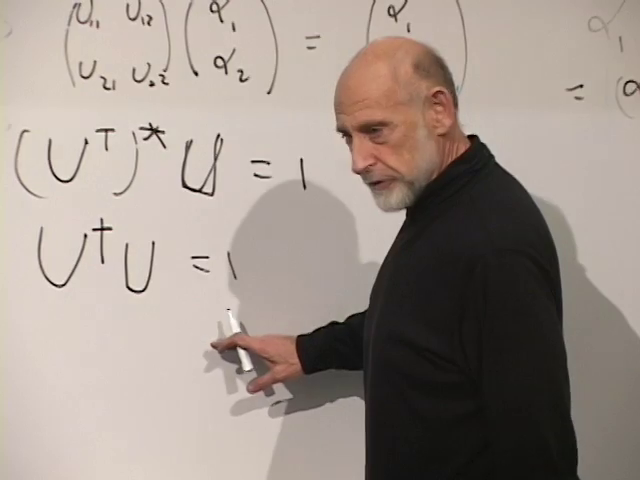
\includegraphics[width=0.62\textwidth]{lecture_03_figure_04.png}
\caption{Ma trận quay spinor thỏa mãn \(U^\dagger U=\boldsymbol 1\).}
\lectureframe{00:27:41}
\end{figure}

Các ma trận thỏa mãn Phương trình~\eqref{eq:l3-unitarity} là unita. Một ma trận phức
\(2\times2\) tổng quát ban đầu có 8 tham số thực. Tính unita là một phương trình ma trận
\(2\times2\) cung cấp 4 ràng buộc thực độc lập,
để lại 4 tham số. Một phép quay không gian chỉ có 3. Cần thêm một
ràng buộc nữa để tách biểu diễn spinor của các phép quay ra khỏi toàn bộ \(U(2)\).

Bốn ràng buộc ấy cũng có thể thấy được nếu xem hai cột của \(U\) như
hai vectơ phức. Mỗi cột phải có chuẩn đơn vị, cho 2 điều kiện thực,
và các cột phải trực giao, cho 1 điều kiện phức hay 2 điều kiện thực.
Tổng cộng là 4. Tham số thứ tư còn lại trong
\(U(2)\) hóa ra sẽ là một pha định thức toàn cục chứ không phải một phép quay không gian mới.

\section{Định thức bằng một và \texorpdfstring{\(SU(2)\)}{SU(2)}}

Điều kiện bổ sung là
\begin{equation}
\det U=1.
\label{eq:l3-det-one}
\end{equation}
Nó tương thích với phép nhân nhóm vì
\begin{equation}
\det(AB)=\det A\,\det B.
\end{equation}
Tích của hai ma trận unita có định thức bằng một lại có định thức bằng một,
và phần tử đơn vị có định thức bằng một. Các ma trận này tạo thành một nhóm con đóng.

Nghịch đảo cũng nằm trong nhóm con. Nếu \(\det U=1\), thì
\begin{equation}
\det U^{-1}=\frac{1}{\det U}=1.
\end{equation}
Vì vậy, áp đặt điều kiện định thức bằng một không loại bỏ phần tử đơn vị,
không phá hỏng tính đóng, cũng không làm mất các nghịch đảo. Nó nhất quán chọn ra một nhóm có ít hơn một tham số liên tục.

Chỉ riêng tính unita đã suy ra
\begin{equation}
\det(U^\dagger U)=
(\det U)^*\det U
=|\det U|^2=1.
\end{equation}
Nó không buộc \(\det U\) phải là \(+1\) hay \(-1\). Định thức unita tổng quát
có thể là bất kỳ pha nào:
\begin{equation}
\det U=e^{i\phi},
\qquad
\det U^\dagger=e^{-i\phi}.
\end{equation}
Điều kiện~\eqref{eq:l3-det-one} cố định pha vốn dĩ tự do này và loại bỏ một
tham số thực.

\begin{classroomqa}
\audiencequestion{Liệu \(U^\dagger U=\boldsymbol 1\), nếu không có điều kiện định thức bằng một, có buộc \(\det U^\dagger\) bằng \(\det U\) hay chỉ có thể là \(+1\) hoặc \(-1\) không?\lecturetimestamp{00:31:21}}
\lecturerresponse{Không. Hai định thức ấy là liên hợp phức của nhau. Chúng có thể là \(e^{i\phi}\) và \(e^{-i\phi}\), mà tích của chúng bằng một. Khi đó ràng buộc unita đặc biệt cố định cả hai bằng một.}
\end{classroomqa}

Các ma trận unita \(n\times n\) tạo thành \(U(n)\). Với \(n=1\), một ma trận unita
chỉ đơn giản là pha \(e^{i\phi}\), cho ta \(U(1)\). Nhóm con định thức bằng một
là nhóm \emph{unita đặc biệt},
\begin{equation}
SU(n)=\{U\in U(n):\det U=1\}.
\end{equation}
Spinor hai thành phần biến đổi dưới tác dụng của \(SU(2)\), một nhóm có 3 tham số.

Ký hiệu ghi lại cả hai ràng buộc: \(U\) nghĩa là unita, còn \(S\)
nghĩa là đặc biệt, tức định thức bằng một. Các nhóm unita đặc biệt này xuất hiện
lặp đi lặp lại vì chúng bảo toàn một tích vô hướng phức đồng thời loại trừ
pha chung độc lập do định thức mang theo.

Xét cục bộ, \(SU(2)\) có cùng đại số quay và cấu trúc phép nhân cần thiết
để quay các trạng thái spin một nửa. Xét toàn cục, phải nhớ đến sự tinh tế đã
tạm hoãn: \(SU(2)\) là phủ đôi của nhóm quay thông thường
\(SO(3)\), nên hai phần tử của \(SU(2)\) tương ứng với một phép quay không gian.
\editorialnote{Phát biểu bằng phủ đôi làm rõ tính hai trị đã được nhắc đến nhưng chưa được triển khai trong nguồn.}

\section{Các phép quay vô cùng bé và các ma trận Pauli}

\begin{classroomqa}
\audiencequestion{Các ma trận spin, hay ma trận Pauli, đi vào cấu trúc này ở đâu?\lecturetimestamp{00:33:16}}
\lecturerresponse{Chúng xuất hiện khi một phần tử nhóm được lấy rất gần phần tử đơn vị, tương ứng với một phép quay qua một góc rất nhỏ. Chúng là các bộ sinh của những phép quay vô cùng bé đó.}
\end{classroomqa}

Bắt đầu với
\begin{equation}
U=\boldsymbol 1+\epsilon M+O(\epsilon^2),
\label{eq:l3-small-u-anti}
\end{equation}
trong đó \(\epsilon\) là thực và nhỏ. Khi đó
\begin{equation}
U^\dagger=\boldsymbol 1+\epsilon M^\dagger+O(\epsilon^2),
\end{equation}
và tính unita cho
\begin{align}
U^\dagger U
 &=\boldsymbol 1+\epsilon(M^\dagger+M)+O(\epsilon^2).
\end{align}
Ở bậc nhất,
\begin{equation}
M^\dagger=-M.
\end{equation}
Vì vậy ma trận \(M\) trong Phương trình~\eqref{eq:l3-small-u-anti} là
phản Hermite.

Chỉ giữ lại các hạng tuyến tính theo \(\epsilon\). Tích
\(\epsilon^2M^\dagger M\) bị bỏ đi vì nó thuộc bậc hai. Đây là
ưu điểm của việc làm việc gần phần tử đơn vị: các điều kiện nhóm phi tuyến
trở thành các điều kiện tuyến tính lên các bộ sinh của chúng.

Thuận tiện hơn nếu tách một thừa số \(i\):
\begin{equation}
U=\boldsymbol 1+i\epsilon H+O(\epsilon^2).
\label{eq:l3-small-u-herm}
\end{equation}
Liên hợp phức biến \(i\) thành \(-i\), nên
\begin{equation}
U^\dagger=\boldsymbol 1-i\epsilon H^\dagger+O(\epsilon^2).
\end{equation}
Bây giờ
\begin{equation}
U^\dagger U
=\boldsymbol 1+i\epsilon(H-H^\dagger)+O(\epsilon^2),
\end{equation}
và tính unita ở bậc nhất đòi hỏi
\begin{equation}
H^\dagger=H.
\end{equation}
Khi đã tách thừa số \(i\) ra, bộ sinh là Hermite.

Phép nhân với \(i\) không làm thay đổi các ma trận vô cùng bé được phép; nó
chỉ thay đổi quy ước dùng để gọi tên bộ sinh. Trong vật lý người ta thường
chọn các bộ sinh Hermite vì các trị riêng của chúng là thực và vì các đại lượng quan sát tương ứng, như mômen góc, là Hermite.

Điều kiện định thức bằng một dẫn đến tính không vết\editorialnote{Trong lời nói, khai triển định thức thoáng làm rối các chỉ số dưới. Số hạng tuyến tính đã hiệu chỉnh là \(A_{11}+A_{22}=\operatorname{tr}A\); các tích ngoài đường chéo chỉ bắt đầu ở bậc hai.}. Với một ma trận
\(2\times2\) nhỏ \(A\),
\begin{equation}
\det(\boldsymbol 1+A)
=
\det
\begin{pmatrix}
1+A_{11}&A_{12}\\
A_{21}&1+A_{22}
\end{pmatrix}.
\end{equation}
Khai triển ra,
\begin{align}
\det(\boldsymbol 1+A)
 &=(1+A_{11})(1+A_{22})-A_{12}A_{21}\\
 &=1+A_{11}+A_{22}+O(A^2)\\
 &=1+\operatorname{tr}A+O(A^2).
\end{align}
Áp dụng điều này cho \(A=i\epsilon H\),
\begin{equation}
\det U=1+i\epsilon\,\operatorname{tr}H+O(\epsilon^2).
\end{equation}
Vì vậy, \(\det U=1\) đòi hỏi
\begin{equation}
\operatorname{tr}H=0.
\end{equation}
Điều kiện vết loại bỏ đúng bộ sinh tỉ lệ với
ma trận đơn vị. Một ma trận Hermite \(2\times2\) tổng quát có 4 tham số thực: 2
phần tử đường chéo thực và 1 phần tử ngoài đường chéo phức. Vết của nó cố định một tổ hợp thực, để lại 3. Điều này khớp với 3 trục mà quanh đó có thể thực hiện một phép quay không gian vô cùng bé.

Vì thế, các bộ sinh vô cùng bé của \(SU(2)\) là các ma trận Hermite \(2\times2\)
không vết. Ba ma trận Pauli tạo thành một cơ sở:
\begin{equation}
\begin{aligned}
\sigma_x&=
\begin{pmatrix}0&1\\1&0\end{pmatrix},
&
\sigma_y&=
\begin{pmatrix}0&-i\\i&0\end{pmatrix},
\\[0.4em]
\sigma_z&=
\begin{pmatrix}1&0\\0&-1\end{pmatrix}.
\end{aligned}
\end{equation}
Mọi bộ sinh đều có thể viết thành
\begin{equation}
H=a_x\sigma_x+a_y\sigma_y+a_z\sigma_z.
\end{equation}
Một phép quay nhỏ quanh trục \(x\) chọn \(\sigma_x\); một phép quay quanh
trục \(y\) chọn \(\sigma_y\); và một phép quay quanh bất kỳ trục nào khác chọn
tổ hợp tuyến tính tương ứng. Trong đơn vị với \(\hbar=1\), các toán tử
spin là
\begin{equation}
S_i=\frac{\sigma_i}{2}.
\end{equation}

Chẳng hạn, một trục nằm chính giữa \(x\) và \(y\) dùng một bộ sinh
tỉ lệ với
\begin{equation}
\frac{\sigma_x+\sigma_y}{\sqrt2}.
\end{equation}
Hướng của vectơ hệ số
\((a_x,a_y,a_z)\) chọn trục quay, còn độ lớn của nó kết hợp với
\(\epsilon\) để đặt góc nhỏ. Đây là mối liên hệ giữa các ma trận spin gặp trong các giao hoán tử mômen góc và các toán tử quay hữu hạn. Cụ thể,
\begin{equation}
[S_x,S_y]=iS_z
\end{equation}
và các hoán vị chu kỳ của nó mã hóa tính không giao hoán đã thấy về mặt hình học.
Phép quay hữu hạn chuẩn thu được bằng cách lấy mũ bộ sinh vô cùng bé\editorialnote{Công thức phép quay hữu hạn dạng hàm mũ là phần hoàn chỉnh chuẩn của cách xây dựng vô cùng bé; nguồn chỉ suy ra các điều kiện của bộ sinh và cơ sở ma trận Pauli của chúng.},
\begin{equation}
U(\hat{\boldsymbol n},\theta)
=\exp\left(-\frac{i\theta}{2}\,
\hat{\boldsymbol n}\cdot\boldsymbol\sigma\right).
\end{equation}
\section{Không gian màu ba trạng thái}

Việc kết hợp các biểu diễn có thể để sau. Giờ ta rời spin trong không gian và quay lại
màu của quark. Một quark vẫn có spin một nửa, nhưng màu của nó là một
độ tự do ba trạng thái độc lập:
\begin{equation}
\lvert r\rangle,\qquad
\lvert g\rangle,\qquad
\lvert b\rangle.
\end{equation}
Một trạng thái màu tổng quát là
\begin{equation}
\begin{aligned}
\lvert q\rangle_{\mathrm{color}}
={}&
\alpha_r\lvert r\rangle
+\alpha_g\lvert g\rangle
+\alpha_b\lvert b\rangle,
\\
&|\alpha_r|^2+|\alpha_g|^2+|\alpha_b|^2=1.
\end{aligned}
\end{equation}
Tương đương,
\begin{equation}
q=
\begin{pmatrix}
\alpha_r\\
\alpha_g\\
\alpha_b
\end{pmatrix}.
\end{equation}
Bình phương độ lớn là các xác suất để có đỏ, lục và lam trong một
cơ sở màu đã chọn. Cùng ký hiệu bộ ba ấy cũng có thể gom ba toán tử trường quark,
\begin{equation}
\psi=
\begin{pmatrix}
\psi_r\\
\psi_g\\
\psi_b
\end{pmatrix}.
\end{equation}

Spin và màu phải được giữ tách biệt về mặt khái niệm. Nhãn spin cho biết trạng thái
biến đổi như thế nào dưới các phép quay của không gian vật lý. Nhãn màu cho biết
nó biến đổi như thế nào dưới một đối xứng nội tại không quay phòng thí nghiệm.
Một trạng thái quark mang cả hai nhãn, dù trong thảo luận hiện tại spin được
lược bỏ để tập trung vào màu.

Viết ba toán tử trường trong một cột không chỉ là việc ghi chép. Nó cho phép
phát biểu đối xứng trong một phương trình ma trận duy nhất. Một phép biến đổi
có thể biến một trường đỏ thành một tổ hợp tuyến tính của các trường đỏ, lục và lam,
giống như một phép quay không gian biến một thành phần vectơ thành một tổ hợp tuyến
tính của các thành phần khác.

Trước hết có thể hình dung các phép biến đổi rời rạc hoán đổi hai màu. Đối xứng
lớn hơn chứa các sự pha trộn liên tục của cả ba. Một ma trận hoán đổi đơn giản
có thể cần kèm theo một pha để làm cho định thức của nó bằng một; khi đó phép
hoán đổi được nhúng vào nhóm unita đặc biệt.

Đối với hai trạng thái cơ sở, phép hoán đổi thuần túy được biểu diễn bởi
\begin{equation}
X=
\begin{pmatrix}0&1\\1&0\end{pmatrix},
\qquad
\det X=-1.
\end{equation}
Nhân toàn bộ ma trận với \(i\) cho
\begin{equation}
\det(iX)=i^2\det X=1.
\end{equation}
Vì vậy, phép hoán đổi rời rạc có thể xuất hiện như một phần tử cụ thể của
nhóm liên tục lớn hơn một khi pha được chọn nhất quán.

\begin{classroomqa}
\audiencequestion{Một ma trận chỉ đơn thuần hoán đổi hai trạng thái cơ sở có định thức sai đối với \(SU(2)\) không?\lecturetimestamp{00:43:46}}
\lecturerresponse{Phép hoán đổi thuần túy có định thức \(-1\). Một thừa số thích hợp của \(i\) cung cấp một đại diện có định thức bằng một, nên phép hoán đổi có thể được bao gồm trong các phép biến đổi unita đặc biệt liên tục.}
\end{classroomqa}

\section{\texorpdfstring{\(SU(3)\)}{SU(3)} và tám bộ sinh màu}

Phép biến đổi màu liên tục là
\begin{equation}
\begin{aligned}
q'&=Uq,
&
U^\dagger U&=\boldsymbol 1,
\\
\det U&=1,
&
U&\in SU(3).
\end{aligned}
\label{eq:l3-su3-action}
\end{equation}
Toán học ở đây là cùng một cấu trúc unita đặc biệt được dùng cho spinor,
nhưng nay \(U\) là \(3\times3\). Đây không phải là một phép quay của không gian vật lý. Nó là
một phép quay trong không gian màu nội tại.

Tính unita bảo toàn chuẩn hóa của trạng thái màu:
\begin{equation}
q^\dagger q
=|\alpha_r|^2+|\alpha_g|^2+|\alpha_b|^2.
\end{equation}
Định thức bằng một loại bỏ hướng pha chung \(U(1)\) khỏi sự pha trộn liên tục.
Các ma trận thu được có thể thực hiện các phép hoán đổi đơn giản, các thay đổi
pha tương đối và các chồng chập liên tục thực sự mà vẫn nằm trong một nhóm đóng.

Việc đếm tham số là trực tiếp. Một ma trận phức \(3\times3\) có 9
phần tử phức, tức 18 tham số thực. Phương trình ma trận
\(U^\dagger U=\boldsymbol 1\) áp đặt 9 điều kiện thực. Điều kiện định thức bằng một
loại bỏ thêm 1 tham số nữa:
\begin{equation}
\dim SU(3)=18-9-1=8.
\end{equation}
Vì vậy, \(SU(3)\) có 8 bộ sinh vô cùng bé độc lập.

9 điều kiện thực của tính unita lại có thể được hiểu theo các cột của
\(U\). Ba cột phức mỗi cột đều phải có chuẩn đơn vị, và mọi cặp
đều phải trực giao. Các điều kiện này loại bỏ 9 trong số 18 tham số thực
ban đầu. Pha định thức loại bỏ tham số thứ 10, còn lại 8.
Đây là bản tương tự ba trạng thái của cách đếm \(8-4-1=3\) cho \(SU(2)\).

Sự xuất hiện của con số tám chính là cùng một sự kiện mà rốt cuộc tạo ra tám loại gluon. Nói rằng không có chín gluon vì ràng buộc định thức đã loại bỏ một phương chỉ là một mẹo ghi nhớ. Chính xác hơn, chín ma trận màu-phản màu phân rã thành một hướng singlet màu, tỉ lệ với ma trận đơn vị, và tám hướng không vết. Tám phần tử sinh không vết tạo thành cấu trúc màu adjoint mà các gluon QCD mang.\editorialnote{Cách trình bày singlet-cộng-octet là phiên bản chính xác tiêu chuẩn của nhận xét về định thức cố ý mang tính gợi ý trong văn bản gốc; việc xây dựng trường chuẩn của nó được để lại cho sau.}

Ở giai đoạn này, mối liên hệ với tám gluon mới là một dấu mốc chỉ đường, chưa phải là một suy dẫn đầy đủ. Để thu được các hạt chuẩn, ta phải nâng đối xứng màu thành đối xứng cục bộ và xác định các trường bù. Điều mà việc đếm tham số đã cho thấy là có tám hướng độc lập mà theo đó một phép biến đổi màu \(SU(3)\) có thể bắt đầu lệch khỏi phần tử đơn vị.

\section{Đối xứng màu ràng buộc QCD}

Phát biểu đối xứng cơ bản là vật lý bất biến dưới phép biến đổi màu trong Phương trình~\eqref{eq:l3-su3-action}. Đây là đối xứng nội tại trung tâm của sắc động lực học lượng tử. Việc trộn các thành phần màu tương tự về mặt hình thức với việc trộn các biên độ spin lên và spin xuống, và đến lượt mình các phép biến đổi spinor đó lại liên hệ với các phép quay của những phương trong không gian, nhưng không được nhầm lẫn ba không gian này với nhau.

Gọi màu là một đối xứng có nghĩa là thay đổi cơ sở màu không làm thay đổi các dự đoán vật lý. Đỏ, xanh lục và xanh lam là những tên gọi tiện dụng cho ba vectơ cơ sở, chứ không phải ba sắc tố có thể quan sát được. Một phép quay \(SU(3)\) tác dụng đồng thời lên các thành phần màu phải giữ nguyên dạng của các định luật. Tính bất biến này không phải là một nét thẩm mỹ tùy chọn; nó là nguyên lý tổ chức của QCD.

Đối xứng ràng buộc Lagrangian. Trong ví dụ \(U(1)\) trước đó, tính bất biến dưới một phép biến đổi pha chung đã buộc các hạng được phép phải chứa các thừa số cân bằng của một trường và liên hợp của nó. Trong QCD, tương tự, mọi hạng đều phải bất biến dưới phép biến đổi màu \(SU(3)\). Yêu cầu đó kéo theo các hệ quả đối với các tương tác, các đại lượng bảo toàn và dạng của trường gluon.

Giả sử một hạng được đề xuất mang một chỉ số màu tự do. Dưới Phương trình~\eqref{eq:l3-su3-action}, chỉ số đó quay, nên bản thân hạng ấy không thể bất biến. Các hạng được phép phải co các chỉ số màu thành những tổ hợp bất biến hoặc dùng các trường chuẩn có phép biến đổi bù lại sự thay đổi đó. Đây là hiệu lực thực tiễn của nguyên lý đối xứng: nó loại trừ các ghép tùy ý và sắp xếp những tương tác còn lại.

Việc xây dựng đầy đủ QCD đòi hỏi thêm một bước nữa: phép biến đổi màu phải được cho phép biến thiên từ điểm này sang điểm khác, và trường chuẩn phải bù cho sự thay đổi cục bộ đó.\editorialnote{Việc địa phương hóa đối xứng màu là cách hoàn chỉnh thông thường trong lý thuyết chuẩn đối với phần thảo luận toàn cục về \(SU(3)\); điều đó không được triển khai trong bài giảng gốc này.} Sự phát triển đó thuộc về giai đoạn tiếp theo. Hiện tại, cấu trúc cốt yếu đã có: một triplet màu chịu tác dụng của một đối xứng unita đặc biệt ba trạng thái với tám phần tử sinh.

Phép tính đã đi sâu vào lý thuyết nhóm đến mức cần thiết cho lúc này. Ta bắt đầu từ các phép quay có thể vẽ trong không gian thông thường, chuyển sang các ma trận tác dụng lên vectơ và spinor, rồi sau đó áp dụng lại cùng lập luận ấy trong một không gian màu nội tại. Ở bước tiếp theo, ta có thể trở lại vật lý hạt với khuôn khổ toán học đã sẵn có, thay vì bắt hình thức luận phải gánh toàn bộ câu chuyện vật lý ngay lập tức.
